\documentclass{math201}

\usepackage[backref]{hyperref} 
\hypersetup{hidelinks}
\usepackage{bookmark}

% =============================================
% Part 0 信息
% =============================================

\mathsetup{
  % 学生姓名
  student = {},
  % 学号
  student-id = {},
  % 院系
  experiment = {GPIO控制LED显示},
  % 专业年级
  discipline = {集成电路设计与集成系统},
  % 日期
  date = {\today},
}

\begin{document}

% =============================================
% Part 1  封面
% =============================================

\makecover

% =============================================
% Part 2 主文档
% =============================================

\section{实验内容}

通过DSP的通用输入输出多路复合器GPIO来控制LED灯的闪烁

\section{实验内容}

\subsection{GPIO的寄存器}

GPIO是通用输入/输出端口,它可以用来控制外部设备,比如LED灯。为了使用GPIO,需要配置一些寄存器,比如:

GpioMuxRegs: 这个寄存器组用来设置GPIO的复用功能,可以选择GPIO是作为普通的I/O口,还是作为其他功能的接口,比如串口、定时器、PWM等。
每个GPIO有一个对应的MUX位,可以通过设置这个位来选择GPIO的功能。
比如,GpioMuxRegs.GPFMUX.bit.MFSRA\_GPIOF11=0; 这句代码就是把GPIOF11设置为通用I/O口,而不是作为MFSRA的接口。

GpioMuxRegs.GPFDIR: 这个寄存器组用来设置GPIO的方向,可以选择GPIO是作为输入口,还是作为输出口。
每个GPIO有一个对应的DIR位,可以通过设置这个位来选择GPIO的方向。比如,GpioMuxRegs.GPFDIR.bit.GPIOF11=1;
这句代码就是把GPIOF11设置为输出口,而不是作为输入口。

\subsection{实验板的LED连接图}

电路原理图如图1所示发光

\begin{figure}[H]  
    \centering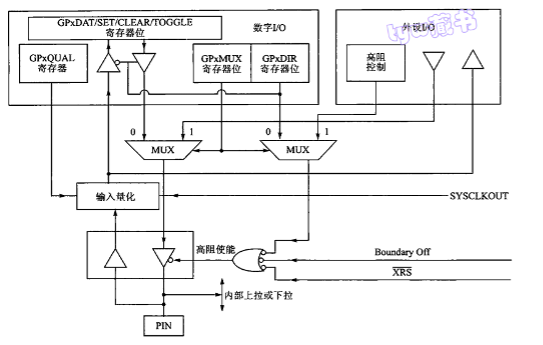
\includegraphics[width=0.8\linewidth]{Picture1.png}  
    \caption{电路原理图}     
    \label{img01}   
\end{figure}

\section{实验步骤}

编写代码,实现LED灯的闪烁,代码如下:

MyDeclaration.h

\inputminted[
    frame=lines,
    framesep=2mm,
    baselinestretch=1.2,
    fontsize=\small,
    linenos
]{C++}{code/MyDeclaration.h}

MyMainDeclaration.h

\inputminted[
    frame=lines,
    framesep=2mm,
    baselinestretch=1.2,
    fontsize=\small,
    linenos
]{C++}{code/MyMainDeclaration.h}

\begin{figure}[H]  
    \centering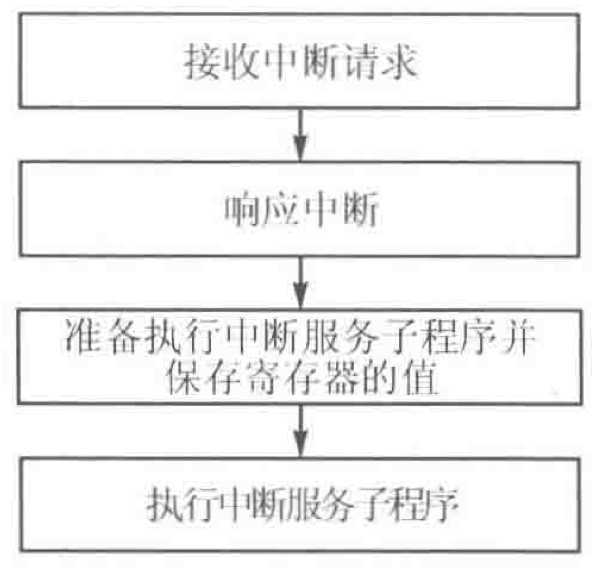
\includegraphics[width=0.8\linewidth]{Picture2.png}  
    \caption{编译调试}     
    \label{img02}   
\end{figure}

\begin{figure}[H]  
    \centering\includegraphics[width=0.8\linewidth]{Picture3.jpg}  
    \caption{下载运行}     
    \label{img03}   
\end{figure}

\begin{figure}[H]  
    \centering\includegraphics[width=0.8\linewidth]{Picture4.jpg}  
    \caption{实验现象}     
    \label{img04}   
\end{figure}

\section{实验小结}

\end{document}
